\chapter{Polarization}

\section{Circular Polarization}

\begin{equation*}
  \left\{
    \begin{aligned}
      & \vec{E}_x \left( z,t \right) = \vec{\imath} E_0 \cos \left( k x - \omega t \right) \\
      & \vec{E}_y \left( z,t \right) = \vec{\jmath} E_0 \sin \left( k x - \omega t \right)
    \end{aligned}
  \right.
  \Rightarrow 
  \begin{aligned}
    \vec{E} = E_0 \left[ \vec{\imath} \cos \left( k x - \omega t \right) + \vec{\jmath} \sin \left( k x - \omega t \right) \right]
  \end{aligned}
  \quad\quad \text{Right-circularly polarized}
\end{equation*}

\begin{equation*}
  \left\{
    \begin{aligned}
      & \vec{E}_x \left( z,t \right) = \vec{\imath} E_0 \cos \left( k z - \omega t \right) \\
      & \vec{E}_y \left( z,t \right) = - \vec{\jmath} E_0 \sin \left( k z - \omega t \right)
    \end{aligned}
  \right.
  \Rightarrow 
  \begin{aligned}
    \vec{E} = E_0 \left[ \vec{\imath} \cos \left( k x - \omega t \right) - \vec{\jmath} \sin \left( k x - \omega t \right) \right]
  \end{aligned}
  \quad\quad \text{Left-circularly polarized}
\end{equation*}

\section{Elliptical Polarization}

\begin{equation*}
  \left\{
    \begin{aligned}
      & \vec{E}_x = E_{0x} \cos \left( k x - \omega t \right) \\
      & \vec{E}_y = E_{0y} \cos \left( k z - \omega t + \epsilon \right)
    \end{aligned}
  \right.
  \quad\quad \text{Elliptical Polarization}
\end{equation*}

\section{Angular Momentum}

\begin{equation*}
  \begin{aligned}
    \dfrac{\md E}{\md t} = \omega M = \omega \dfrac{\md L}{\md t}  
  \end{aligned}
  \Rightarrow 
  \begin{aligned}
    L = \dfrac{E}{\omega} = \dfrac{h \nu}{\omega} = \pm \hbar = 
  \end{aligned}
  \left\{
    \begin{aligned}
      & - \hbar \quad\quad \text{Right-circularly polarized} \\
      & + \hbar \quad\quad \text{Left-circularly polarized}
    \end{aligned}
  \right.
\end{equation*}

\section{Malus's Law}

\begin{figure}[H]
  \centering
  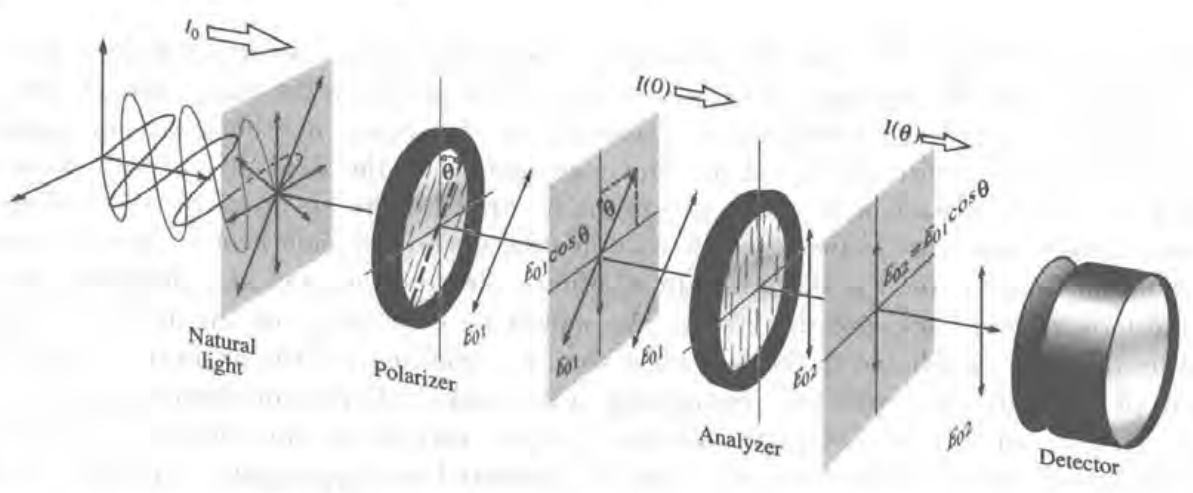
\includegraphics[width=0.7\linewidth]{figures/Malus}
  \label{fig:}
\end{figure}

\begin{equation*}
  \left\{
    \begin{aligned}
      & E_{02} = E_{01} \cos \theta \\
      & I \left( \theta \right) = \dfrac{c \varepsilon_0}{2} E_{01}^2 \cos^2 \theta = I \left( 0 \right) \cos^2 \theta
    \end{aligned}
  \right.
\end{equation*}

\section{Dichroism}

\subsection{The Wire-Grid Polarizer and Dichroic Crystals, Polaroid}

\begin{figure}[H]
  \centering
  \begin{subfigure}{.4\textwidth}
    \centering
    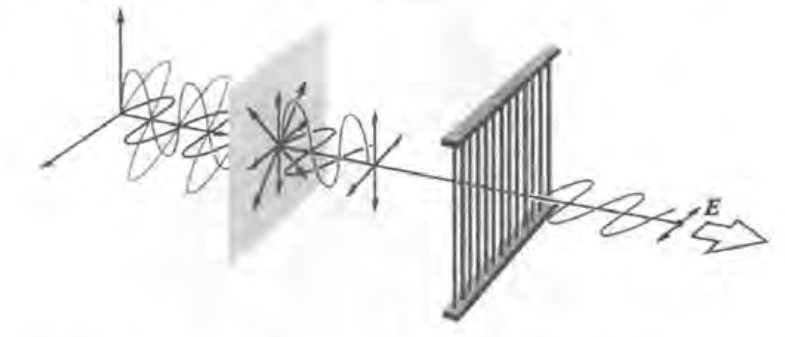
\includegraphics[width=\linewidth]{figures/WireGrid}
    \label{fig:}
  \end{subfigure}
  \begin{subfigure}{.18\textwidth}
    \centering
    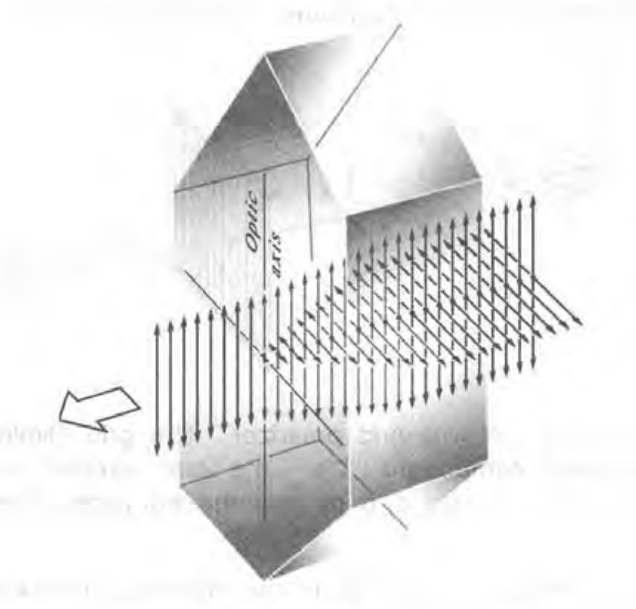
\includegraphics[width=\linewidth]{figures/Dichroic-Crystals}
    \label{fig:}
  \end{subfigure}
  \label{fig:}
  \begin{subfigure}{.4\textwidth}
    \centering
    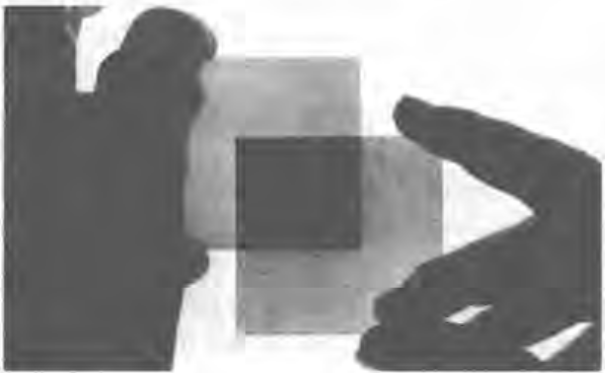
\includegraphics[width=0.6\linewidth]{figures/Polaroid}
    \label{fig:}
  \end{subfigure}
  \label{fig:}
\end{figure}

\section{Birefringent Crystals}

\begin{figure}[H]
  \centering
  \begin{subfigure}{.5\textwidth}
    \centering
    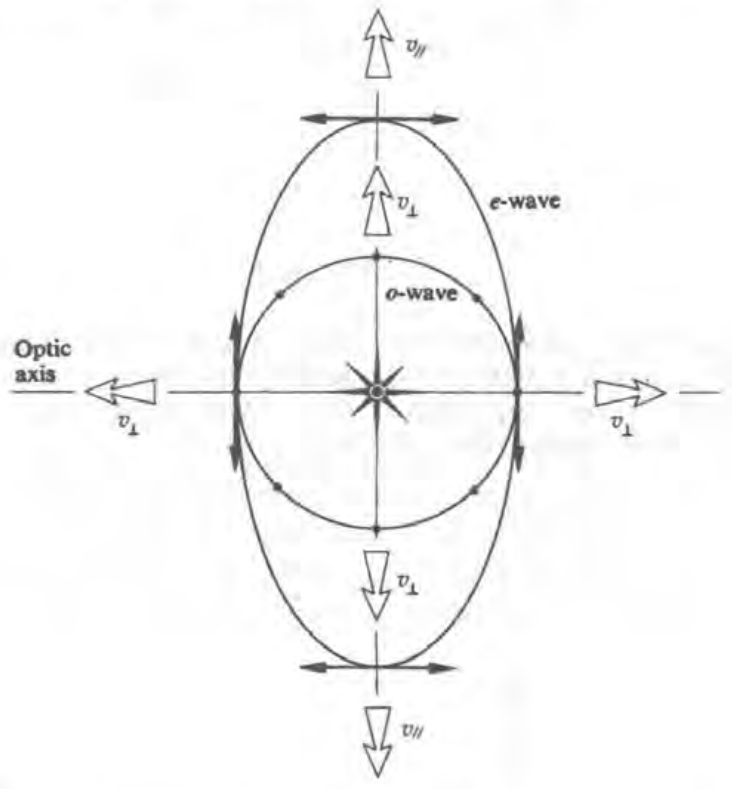
\includegraphics[width=0.7\linewidth]{figures/negative-uniaxial}
    \caption{$v_{\perp} < v_{\parallel} \Rightarrow n_o > n_e \Rightarrow \text{negative uniaxial}$}
    \label{fig:}
  \end{subfigure}%
  \begin{subfigure}{.5\textwidth}
    \centering
    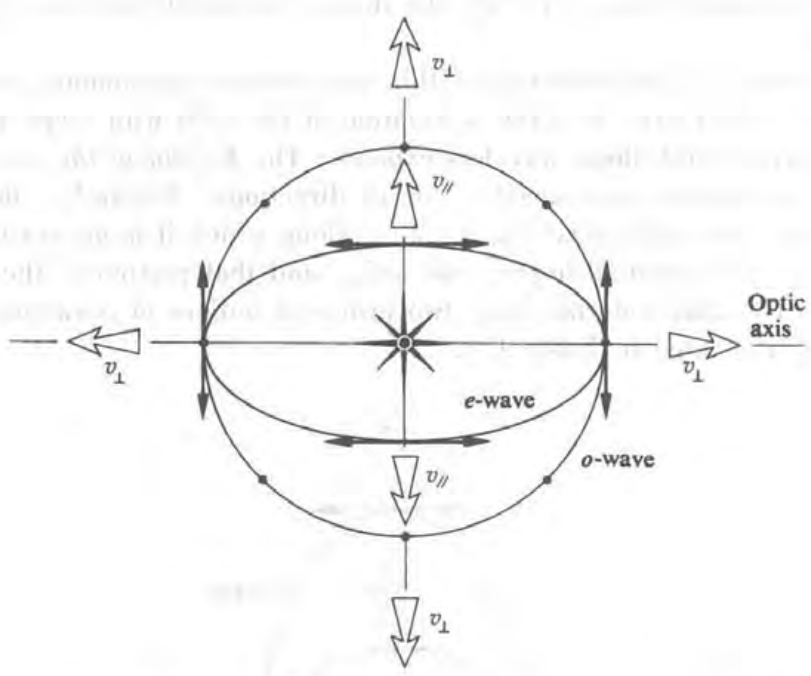
\includegraphics[width=0.7\linewidth]{figures/positive-uniaxial}
    \caption{$v_{\perp} > v_{\parallel} \Rightarrow n_o > n_e \Rightarrow \text{positive uniaxial}$}
    \label{fig:}
  \end{subfigure}
  \caption{negative and positive uniaxial}
  \label{fig:}
\end{figure}

\section{Polarizers}

\begin{figure}[H]
  \centering
  \begin{subfigure}{.5\textwidth}
    \centering
    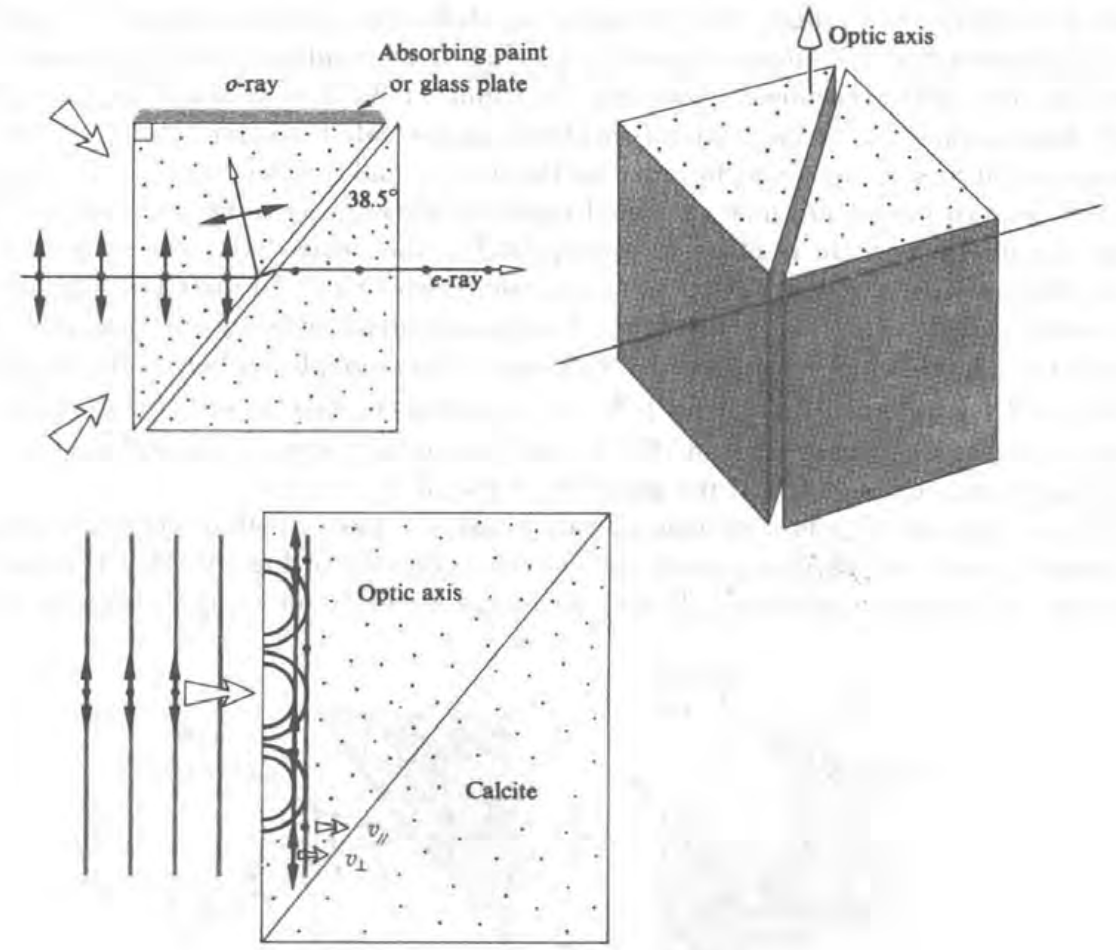
\includegraphics[width=0.75\linewidth]{figures/Polarizer1}
    \caption{The Glan-Foucault Prism}
    \label{fig:}
  \end{subfigure}%
  \begin{subfigure}{.5\textwidth}
    \centering
    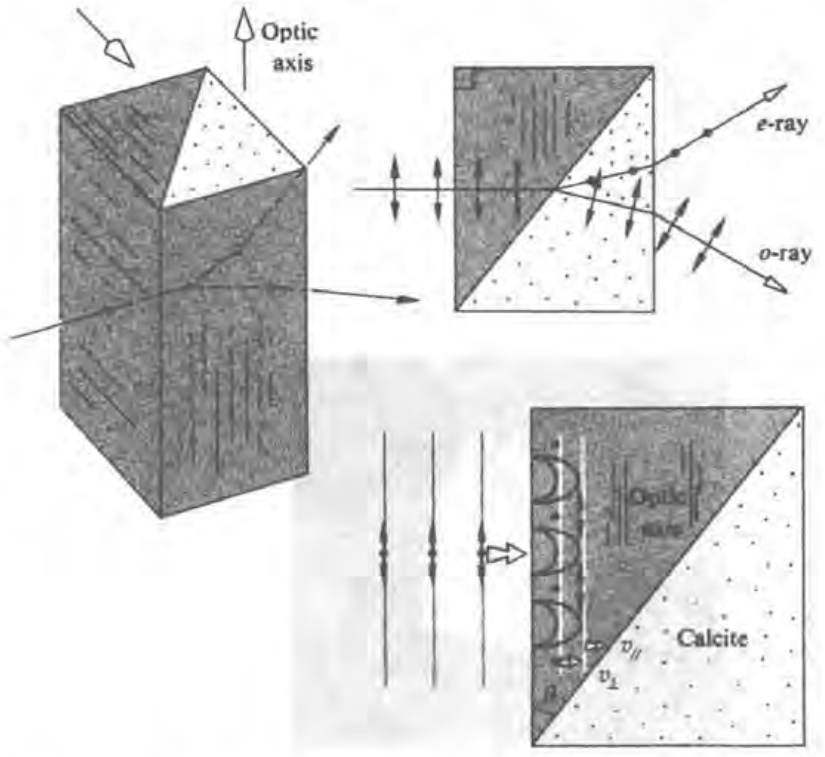
\includegraphics[width=0.75\linewidth]{figures/Polarizer2}
    \caption{The Wollaston Prism}
    \label{fig:}
  \end{subfigure}
  \caption{Tow Birefringent Polarizers}
  \label{fig:}
\end{figure}

\section{Scattering and Polarization}

\begin{figure}[H]
  \centering
  \begin{subfigure}{.6\textwidth}
    \centering
    \includegraphics[width=\linewidth]{figures/Scattering-Polarization-1}
    \label{fig:}
  \end{subfigure}%
  \begin{subfigure}{.3\textwidth}
    \centering
    \includegraphics[width=0.9\linewidth]{figures/Scattering-Polarization-2}
    \label{fig:}
  \end{subfigure}
  \label{fig:}
\end{figure}

\section{Retarders}

\begin{figure}[H]
  \centering
  \begin{subfigure}{.5\textwidth}
    \centering
    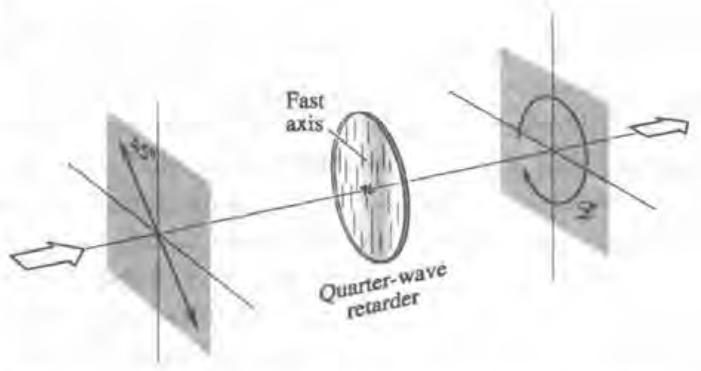
\includegraphics[width=0.8\linewidth]{figures/Retarder}
    \caption{Quarter-wave Retarder}
    \label{fig:}
  \end{subfigure}%
  \begin{subfigure}{.5\textwidth}
    \centering
    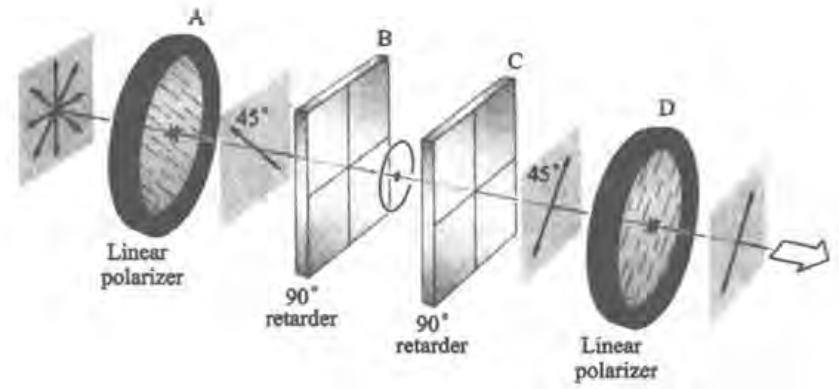
\includegraphics[width=0.9\linewidth]{figures/Retarder2}
    \caption{Two Linear Polarizers and Two Quarter-wave Retarders}
    \label{fig:}
  \end{subfigure}
  \label{fig:}
  \caption{Quarter-wave Retarder and its Application}
\end{figure}

\begin{equation*}
  \begin{aligned}
    d \left( n_o - n_e \right) = \dfrac{4 m + 1}{4} \lambda_0 
  \end{aligned}
\end{equation*}


%%% Local Variables:
%%% mode: latex
%%% TeX-master: "Optics"
%%% End:
